\documentclass{article}
\usepackage[T1]{fontenc}
\usepackage{lmodern}
\usepackage{graphicx}
\usepackage{amsmath,amssymb}
\usepackage[a4paper,margin=2cm]{geometry}
\usepackage[absolute,overlay]{textpos}
\setlength{\TPHorizModule}{1mm}
\setlength{\TPVertModule}{1mm}
\usepackage[indonesian]{babel}
\usepackage{hyperref}
\setlength{\emergencystretch}{2em}
% unit: Halaman 81

\begin{document}

% === Halaman 81 (llm) ===

\vspace{213.84mm}

Demo Playfair cipher online: \url{https://planetcalc.com/7751/}

% deskripsi: Screenshot alat kalkulator online Playfair cipher yang menunjukkan teks input, keyword, proses enkripsi, kotak Playfair (Playfair square), dan teks hasil transformasi.
% bbox normalisasi: [0.7300, 0.1400, 0.9000, 0.8600]
\begin{textblock*}{35.70mm}(153.30mm,41.58mm)
\noindent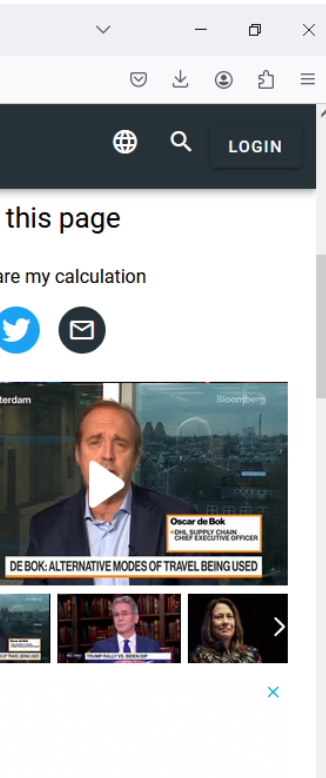
\includegraphics[width=35.70mm,height=213.84mm]{../../images/llm/page_081_img_01.png}%
\end{textblock*}

\end{document}
